% !TEX program = lualatex

\documentclass{beamer}

\title{Modelos Generativos Profundos}
\subtitle{Clase 1: Introducción}
\author{Fernando Fêtis Riquelme}
\institute{
    Facultad de Ciencias Físicas y Matemáticas\\
    Universidad de Chile
}
\date{Otoño, 2026}
\titlegraphic{\hfill
\includegraphics[height=1.2cm]{images/fcfm.pdf}}

\usetheme{metropolis}
\setbeamercovered{transparent}
\newcommand{\insertimage}[2]{%
    \par\noindent\hspace*{-\leftmargini}\centering\includegraphics[width=#2\textwidth]{images/#1}\par
}
\renewcommand{\raggedright}{\leftskip=0pt \rightskip=0pt plus 0cm}

\begin{document}

\begin{frame}
    \titlepage
\end{frame}

\begin{frame}{Clase de hoy}
    \tableofcontents
\end{frame}

\section{Overview de los modelos generativos modernos}

\begin{frame}{Qué puede generar un modelo generativo}
    \begin{itemize}
        \item<1> Creación y modificación de imágenes.
        \only<1>{\insertimage{image_1}{0.7}}
        \item<2> Generación de sonido y video.
        \only<2>{\insertimage{image_2}{1}}
        \item<3> Simulaciones de juegos.
        \only<3>{\insertimage{image_3}{0.9}}
        \item<4> Robótica potenciada por LLMs.
        \only<4>{\insertimage{image_4}{0.9}}
        \item<5> Predicción de estructuras moleculares.
        \only<5>{\insertimage{image_5}{1}}
        \item<6> Agentes autónomos.
        \only<6>{\insertimage{image_6}{1}}
        \item<7> Investigaciones científicas.
        \only<7>{\insertimage{image_7}{0.8}}
    \end{itemize}
\end{frame}

\begin{frame}{Perspectivas para estudiar los modelos generativos}
    Los modelos generativos actuales pueden ser estudiados desde distintos ángulos.
    \begin{itemize}
        \item<1> Perspectiva económica y política.
        \item<2> Perspectiva ética.
        \item<3> Interés filosófico.
        \item<4> Interés teórico.
    \end{itemize}
\end{frame}

\begin{frame}{Paradigmas modernos de la IA generativa}
    \begin{enumerate}
        \item<1> Modelos autorregresivos.
        \item<2> Redes generativas adversarias.
        \item<3> Autoencoders variacionales.
        \item<4> Modelos basados en score.
        \item<5> Modelos basados en flujo.
        \item<6> Modelos de difusión.
    \end{enumerate}
\end{frame}

\section{Requisitos y evaluaciones del curso}

\begin{frame}{Requisitos del curso}
    Si bien el curso es autocontenido, se asumen algunos conocimientos previos.
    \begin{itemize}
        \item \textbf{Probabilidades:} distribuciones clásicas, variables independientes, probabilidad condicional, regla de Bayes, marginalización, verosimilitud, esperanza, etc.
        \item \textbf{PyTorch:} creación de datasets, redes fully-connected, redes convolucionales, entrenamiento de modelos, etc.
    \end{itemize}
    Se realizará un repaso breve de estos temas en la siguiente clase.
\end{frame}

\begin{frame}{Evaluaciones}
    Hay dos tipos de evaluación en el curso.
    \begin{itemize}
        \item \textbf{Tareas (60\%):} 3 en total.
        \item \textbf{Controles de lectura (40\%):} 7 en total.
    \end{itemize}
    Ambos items deben ser aprobados por separado para aprobar el curso.
\end{frame}

\begin{frame}{Evaluaciones}
    Algunas consideraciones.
    \begin{itemize}
        \item Las tareas se realizan de forma individual.
        \item Cada tarea tiene 2 semanas de plazo. \textbf{No se dará plazo adicional}.
        \item Los controles de lectura se realizan en clases.
        \item De los 7 controles de lectura, se elimina 1 para el cálculo de la nota.
        \item Se pueden usar herramientas tipo ChatGPT para las tareas.
    \end{itemize}
\end{frame}

\section{Calendario y bibliografía}

\begin{frame}{Calendario de clases}
    \begin{itemize}
        \item<1> Introducción (2 semanas).
        \item<1> Modelos autorregresivos (3 semanas).
        \item<2> Redes generativas adversarias (2 semanas).
        \item<2> Autoencoders variacionales (2 semanas).
        \item<2> Flujos normalizantes (1 semana).
        \item<3> Modelos basados en score (1 semana).
        \item<3> Modelos de difusión (2 semanas).
        \item<3> Modelos a tiempo continuo (2 semanas).
    \end{itemize}
\end{frame}

\begin{frame}{Libros de referencia}
    Hay 3 libros que se recomiendan para el curso. El 1º sirve como introducción a cada tema, el 2º contiene la formalidad matemática, y el 3º contiene implementaciones en PyTorch.
    \vspace{0.3cm}
    \begin{center}
        \href{https://www.oreilly.com/library/view/generative-deep-learning/9781098134174/}{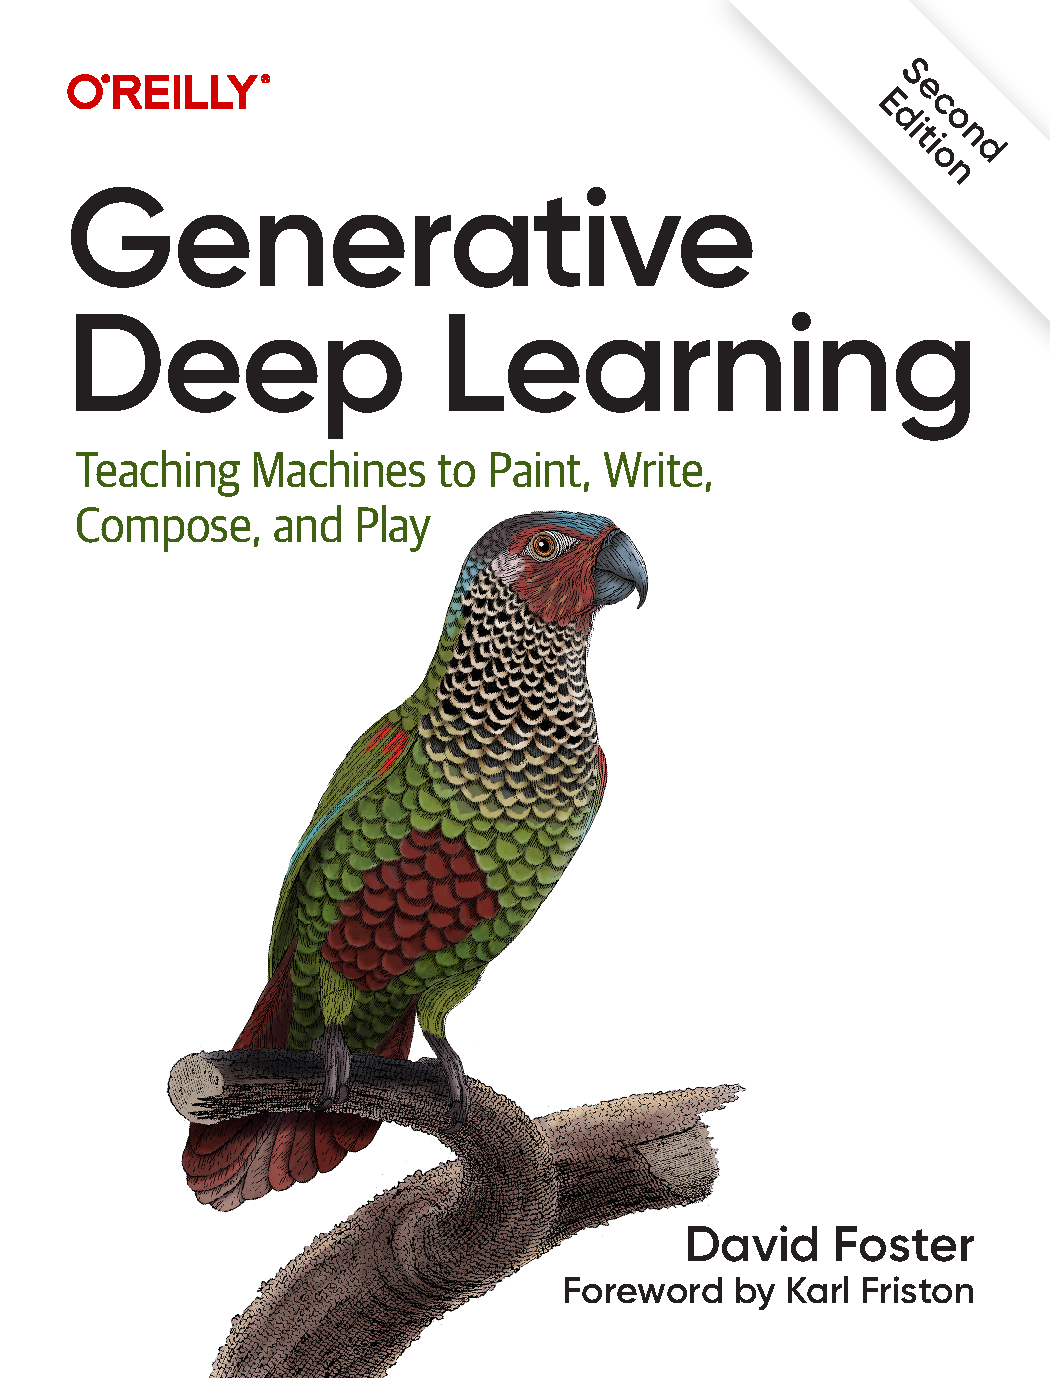
\includegraphics[width=0.3\textwidth]{images/foster.pdf}}
        \href{https://probml.github.io/pml-book/book2.html}{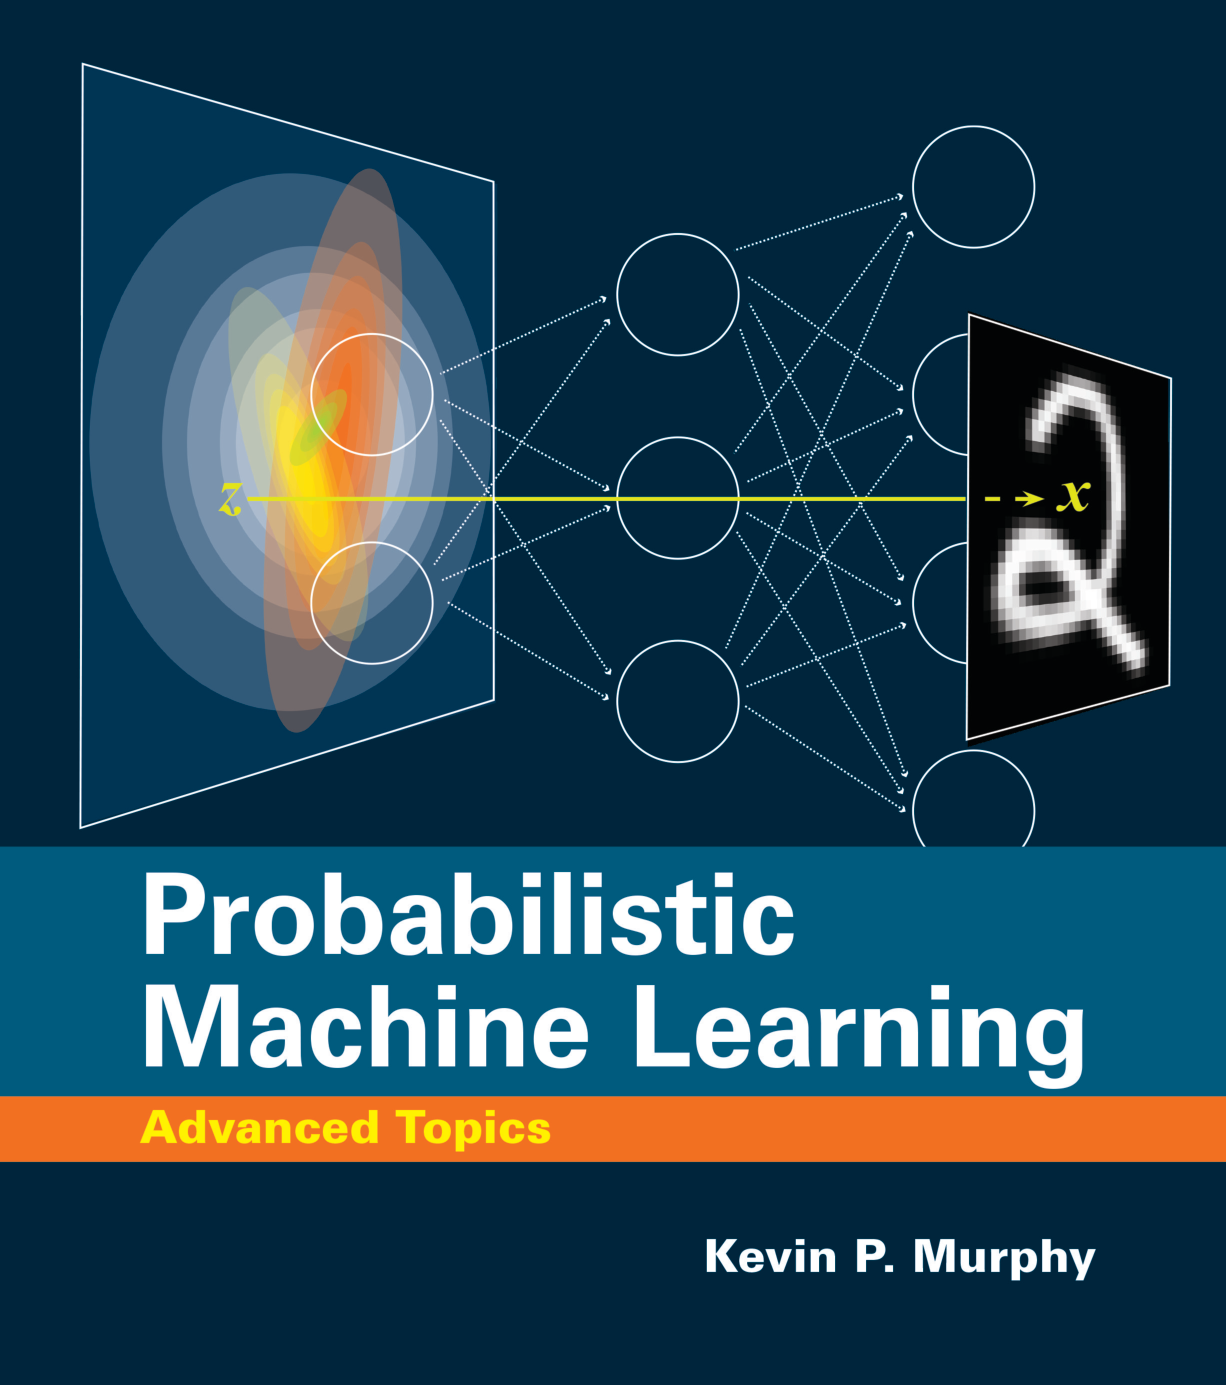
\includegraphics[width=0.3\textwidth]{images/murphy.pdf}}
        \href{https://link.springer.com/book/10.1007/978-3-031-64087-2}{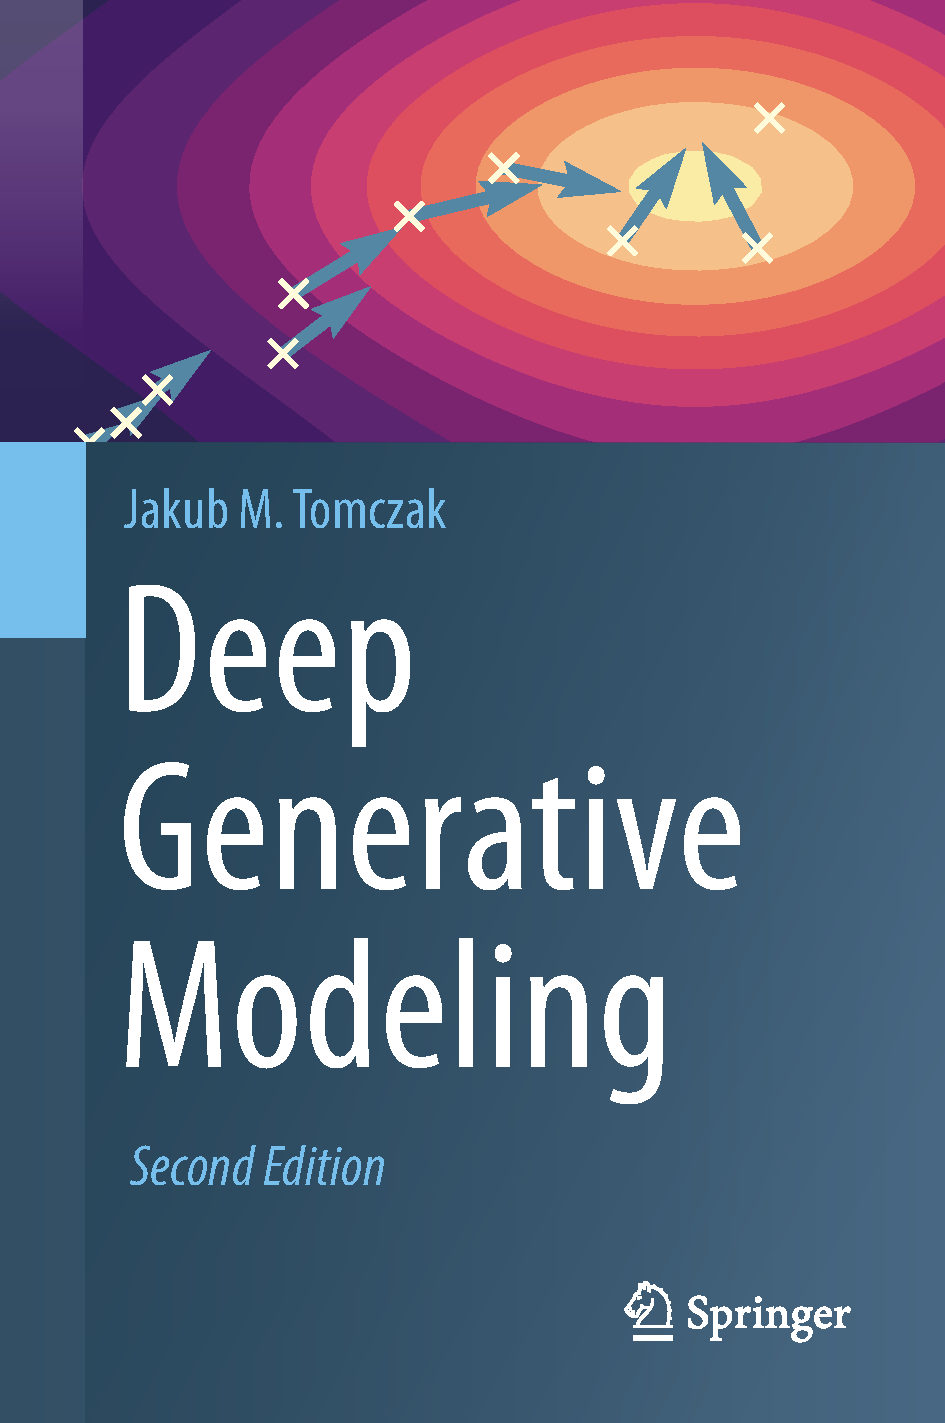
\includegraphics[width=0.3\textwidth]{images/tomczak.pdf}}
    \end{center}
\end{frame}

\begin{frame}{Próxima clase}
    En la próxima clase.
    \begin{itemize}
        \item Repaso de conceptos de probabilidades.
        \item Repaso de conceptos de redes neuronales.
    \end{itemize}
\end{frame}

\begin{frame}
    \centering
    \Large{Modelos Generativos Profundos}\\
    \large{Clase 1: Introducción}
\end{frame}

\end{document}
